\let\negmedspace\undefined
\let\negthickspace\undefined
\documentclass[journal,12pt,onecolumn]{IEEEtran}
\usepackage{cite}
\usepackage{amsmath,amssymb,amsfonts,amsthm}
\usepackage{algorithmic}
\usepackage{graphicx}
\usepackage{textcomp}
\usepackage{xcolor}
\usepackage{txfonts}
\usepackage{listings}
\usepackage{enumitem}
\usepackage{mathtools}
\usepackage{gensymb}

\usepackage{tkz-euclide} % loads  TikZ and tkz-base
\usepackage{listings}
\usetikzlibrary{positioning,arrows,shapes}


\newtheorem{theorem}{Theorem}[section]
\newtheorem{problem}{Problem}
\newtheorem{proposition}{Proposition}[section]
\newtheorem{lemma}{Lemma}[section]
\newtheorem{corollary}[theorem]{Corollary}
\newtheorem{example}{Example}[section]
\newtheorem{definition}[problem]{Definition}
%\newtheorem{thm}{Theorem}[section] 
%\newtheorem{defn}[thm]{Definition}
%\newtheorem{algorithm}{Algorithm}[section]
%\newtheorem{cor}{Corollary}
\newcommand{\BEQA}{\begin{eqnarray}}
\newcommand{\EEQA}{\end{eqnarray}}
\newcommand{\system}[1]{\stackrel{#1}{\rightarrow}}

\newcommand{\define}{\stackrel{\triangle}{=}}
\theoremstyle{remark}
\newtheorem{rem}{Remark}
%\bibliographystyle{ieeetr}
\begin{document}
%
\providecommand{\pr}[1]{\ensuremath{\Pr\left(#1\right)}}
\providecommand{\prt}[2]{\ensuremath{p_{#1}^{\left(#2\right)} }}        % own macro for this question
\providecommand{\qfunc}[1]{\ensuremath{Q\left(#1\right)}}
\providecommand{\sbrak}[1]{\ensuremath{{}\left[#1\right]}}
\providecommand{\lsbrak}[1]{\ensuremath{{}\left[#1\right.}}
\providecommand{\rsbrak}[1]{\ensuremath{{}\left.#1\right]}}
\providecommand{\brak}[1]{\ensuremath{\left(#1\right)}}
\providecommand{\lbrak}[1]{\ensuremath{\left(#1\right.}}
\providecommand{\rbrak}[1]{\ensuremath{\left.#1\right)}}
\providecommand{\cbrak}[1]{\ensuremath{\left\{#1\right\}}}
\providecommand{\lcbrak}[1]{\ensuremath{\left\{#1\right.}}
\providecommand{\rcbrak}[1]{\ensuremath{\left.#1\right\}}}
\newcommand{\sgn}{\mathop{\mathrm{sgn}}}
\providecommand{\abs}[1]{\left\vert#1\right\vert}
\providecommand{\res}[1]{\Res\displaylimits_{#1}} 
\providecommand{\norm}[1]{\left\lVert#1\right\rVert}
%\providecommand{\norm}[1]{\lVert#1\rVert}
\providecommand{\mtx}[1]{\mathbf{#1}}
\providecommand{\mean}[1]{E\left[ #1 \right]}
\providecommand{\cond}[2]{#1\middle|#2}
\providecommand{\fourier}{\overset{\mathcal{F}}{ \rightleftharpoons}}
\newenvironment{amatrix}[1]{%
  \left(\begin{array}{@{}*{#1}{c}|c@{}}
}{%
  \end{array}\right)
}
%\providecommand{\hilbert}{\overset{\mathcal{H}}{ \rightleftharpoons}}
%\providecommand{\system}{\overset{\mathcal{H}}{ \longleftrightarrow}}
	%\newcommand{\solution}[2]{\textbf{Solution:}{#1}}
\newcommand{\solution}{\noindent \textbf{Solution: }}
\newcommand{\cosec}{\,\text{cosec}\,}
\providecommand{\dec}[2]{\ensuremath{\overset{#1}{\underset{#2}{\gtrless}}}}
\newcommand{\myvec}[1]{\ensuremath{\begin{pmatrix}#1\end{pmatrix}}}
\newcommand{\mydet}[1]{\ensuremath{\begin{vmatrix}#1\end{vmatrix}}}
\newcommand{\myaugvec}[2]{\ensuremath{\begin{amatrix}{#1}#2\end{amatrix}}}
\providecommand{\rank}{\text{rank}}
\providecommand{\pr}[1]{\ensuremath{\Pr\left(#1\right)}}
\providecommand{\qfunc}[1]{\ensuremath{Q\left(#1\right)}}
	\newcommand*{\permcomb}[4][0mu]{{{}^{#3}\mkern#1#2_{#4}}}
\newcommand*{\perm}[1][-3mu]{\permcomb[#1]{P}}
\newcommand*{\comb}[1][-1mu]{\permcomb[#1]{C}}
\providecommand{\qfunc}[1]{\ensuremath{Q\left(#1\right)}}
\providecommand{\gauss}[2]{\mathcal{N}\ensuremath{\left(#1,#2\right)}}
\providecommand{\diff}[2]{\ensuremath{\frac{d{#1}}{d{#2}}}}
\providecommand{\myceil}[1]{\left \lceil #1 \right \rceil }
\newcommand\figref{Fig.~\ref}
\newcommand\tabref{Table~\ref}
\newcommand{\sinc}{\,\text{sinc}\,}
\newcommand{\rect}{\,\text{rect}\,}
%%
%	%\newcommand{\solution}[2]{\textbf{Solution:}{#1}}
%\newcommand{\solution}{\noindent \textbf{Solution: }}
%\newcommand{\cosec}{\,\text{cosec}\,}
%\numberwithin{equation}{section}
%\numberwithin{equation}{subsection}
%\numberwithin{problem}{section}
%\numberwithin{definition}{section}
%\makeatletter
%\@addtoreset{figure}{problem}
%\makeatother

%\let\StandardTheFigure\thefigure
\let\vec\mathbf

\bibliographystyle{IEEEtran}





\bigskip

\renewcommand{\thefigure}{\theenumi}
\renewcommand{\thetable}{\theenumi}
%\renewcommand{\theequation}{\theenumi}


\title{GATE 2023 EC}
\author{Praful Kesavadas\\ EE23BTECH11049}
\maketitle

\textbf{Question: 42} In the following block diagram, $R(s)$ and $D(s)$ are two inputs. The output Y(s) is expressed as $Y(s) = G_1(s)R(s) + G_2(s)D(s).$\\
$G_1(s)$ and $G_2(s)$ are given by\\
\begin{figure}[htbp]
\centering
\begin{tikzpicture}[thick,font=\large]
  \draw[-latex] (0,0) -- (2,0);
  \node at (-0.5,0) {$R\brak{s}$};
  \draw (2.5,0) circle [radius = 0.5cm];
  \node[above]  at (1.8,0) {+};
  \node[below] at (1.9,-0.3) {-};
  \draw[-latex] (3,0) -- (5,0);
  \draw (5.5,0) circle [radius=0.5cm];
  \node[above]at (4.8,0){+};
  \node[below]at (4.9,-0.3){-};
  \draw[-latex] (5.5, 2) -- (5.5,0.5);
  \node[above] at (5.5,2) {$D\brak{s}$};
  \draw[-latex] (6,0) -- (7,0);
  \draw (7,-0.5) rectangle (9, 0.5);
  \node at (8,0) {$G\brak{s}$};
  \draw[-latex] (9,0) -- (11,0);
  \node at (11.5,0) {$Y\brak{s}$};
  \draw[-] (10,0) -- (10,-3.5);
  \draw[-latex] (10,-2) -- (9,-2);
  \draw (9, -2.5) rectangle (7,-1.5);
  \node at (8,-2) {$H\brak{s}$};
  \draw[-] (7,-2) -- (5.5,-2);
  \draw[-latex] (5.5,-2) -- (5.5, -0.5);
  \draw[-] (10,-3.5) -- (2.5, -3.5);
  \draw[-latex] (2.5, -3.5) -- (2.5, -0.5);
\end{tikzpicture}

\end{figure}\\
\begin{enumerate}[label=\alph*)]
\item $G_1\brak{s} = \frac{G\brak{s}}{1+G\brak{s}+G\brak{s}H\brak{s}}$ and $G_2\brak{s} = \frac{G\brak{s}}{1+ G\brak{s}+G\brak{s}H\brak{s}}$\\
\item $G_1\brak{s} = \frac{G\brak{s}}{1+G\brak{s}+H\brak{s}}$ and $G_2\brak{s} = \frac{G\brak{s}}{1+ G\brak{s}+H\brak{s}}$\\
\item $G_1\brak{s} = \frac{G\brak{s}}{1+G\brak{s}+H\brak{s}}$ and $G_2\brak{s} = \frac{G\brak{s}}{1+ G\brak{s}+G\brak{s}H\brak{s}}$\\
\item $G_1\brak{s} = \frac{G\brak{s}}{1+G\brak{s}+G\brak{s}H\brak{s}}$ and $G_2\brak{s} = \frac{G\brak{s}}{1+ G\brak{s}+H\brak{s}}$\\
\end{enumerate}
\solution\\
Let $Y\brak{s}= Y_1\brak{s} + Y_2\brak{s}$, where $Y_1\brak{s}$= output considering only $R\brak{s}$, $Y_2\brak{s}$ = Output considering only $D\brak{s}$\\

When only R(s) is present:
\begin{figure}[htbp]
\centering
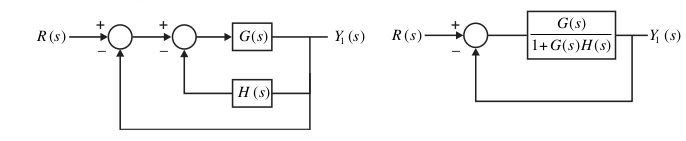
\includegraphics[width=\columnwidth]{figs/Rs.png}
\end{figure}\\
\begin{align}
\frac{Y_1\brak{s}}{R\brak{s}} &= \frac{\frac{G\brak{s}}{1+ G\brak{s}H\brak{s}}}{1+ \frac{G\brak{s}}{1+G\brak{s}H\brak{s}}}\\
Y_1\brak{s} &= \left[\frac{G\brak{s}}{1+ G\brak{s}+ G\brak{s}H\brak{s}}\right] R\brak{s}
\end{align}
Hence,
\begin{align}
 G_1\brak{s} = \frac{G\brak{s}}{1+G\brak{s}+G\brak{s}H\brak{s}}
\end{align}
When only $D\brak{s}$ is present,
\begin{figure}[htbp]
\centering
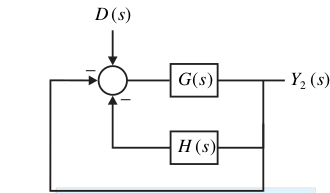
\includegraphics[width=0.49\columnwidth]{figs/Ds1.png}
\begin{circuitikz}[scale=1.5]
    \draw
    (0,0) to[short, -*] node[pos=0] {$\textgreater$} node[pos=0.7, below=1mm] {$y_1$} node[pos=0,above=1.5mm] {$1$} (1,0) to [short,-*] node[pos=0] {$\textgreater$} node[pos=0,above=2mm] {$G(s)$} (3,0) to [short,-] (3.5,0);
    
    \draw (3,0) to [out=-90,in=-90] node[pos=0.5] {$\textless$} node[pos=0.4,below=2mm] {$-(1+H(s))$} (1,0);
    \node[left] at (0,0) {$D(s)$};
    \node[right] at (3.5,0) {$Y_2(s)$};
\end{circuitikz}

\end{figure}\\
\begin{align}
\frac{Y_2\brak{s}}{D\brak{s}} &= \frac{G\brak{s}}{1+G\brak{s}\left[1+ H\brak{s}\right]}\\
Y_2\brak{s}&= \left[ \frac{G\brak{s}}{1+G\brak{s}\left[1+H\brak{s}\right]}\right]D\brak{s}
\end{align}
Hence, 
\begin{align}
G_2\brak{s} = \frac{G\brak{s}}{1+ G\brak{s}+ G\brak{s}H\brak{s}}
\end{align}
Option (a) is correct
\end{document}
